\clearpage
\myparagraph{\olly}

Так как этот пример немного запутанный, попробуем оттрассировать его в \olly.

\olly может распознавать подобные switch()-конструкции, так что он добавляет полезные комментарии.
\EAX в начале равен 2, это входное значение функции: 

\begin{figure}[H]
\centering
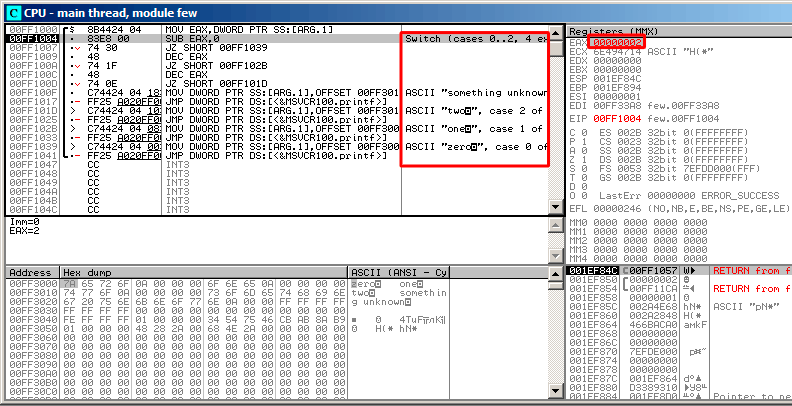
\includegraphics[scale=\FigScale]{patterns/08_switch/1_few/olly1.png}
\caption{\olly: \EAX содержит первый (и единственный) аргумент функции}
\label{fig:switch_few_olly1}
\end{figure}

\clearpage
0 отнимается от 2 в \EAX. 
Конечно же, \EAX всё ещё содержит 2.
Но флаг \ZF теперь 0, что означает, что последнее вычисленное значение не было нулевым:

\begin{figure}[H]
\centering
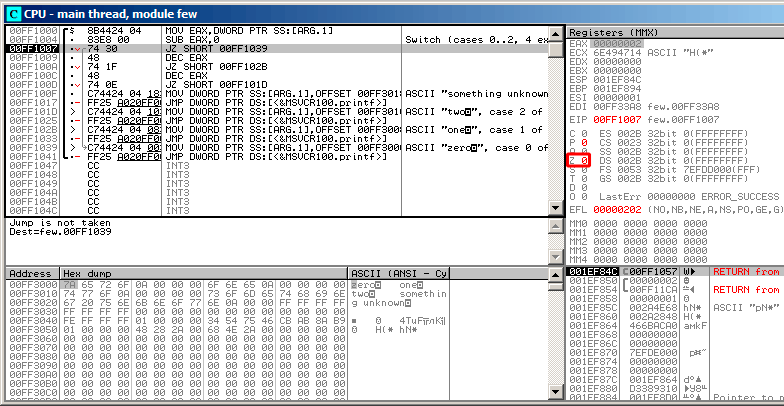
\includegraphics[scale=\FigScale]{patterns/08_switch/1_few/olly2.png}
\caption{\olly: \SUB исполнилась}
\label{fig:switch_few_olly2}
\end{figure}

\clearpage
\DEC исполнилась и \EAX теперь содержит 1. 
Но 1 не ноль, так что флаг \ZF всё ещё 0:

\begin{figure}[H]
\centering
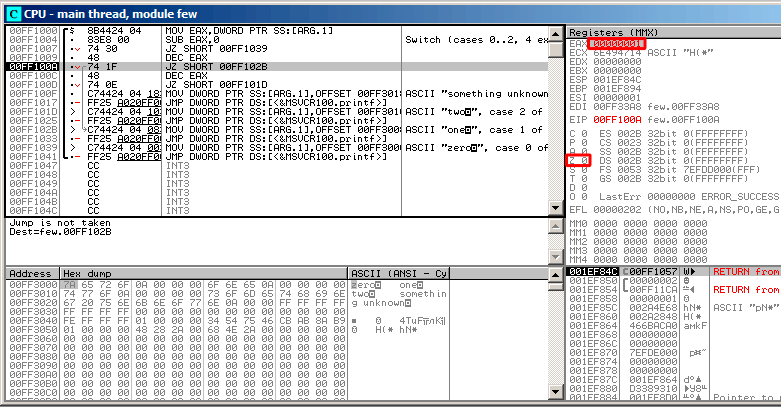
\includegraphics[scale=\FigScale]{patterns/08_switch/1_few/olly3.png}
\caption{\olly: первая \DEC исполнилась}
\label{fig:switch_few_olly3}
\end{figure}

\clearpage
Следующая \DEC исполнилась. 
\EAX наконец 0 и флаг \ZF выставлен, потому что результат~--- ноль:

\begin{figure}[H]
\centering
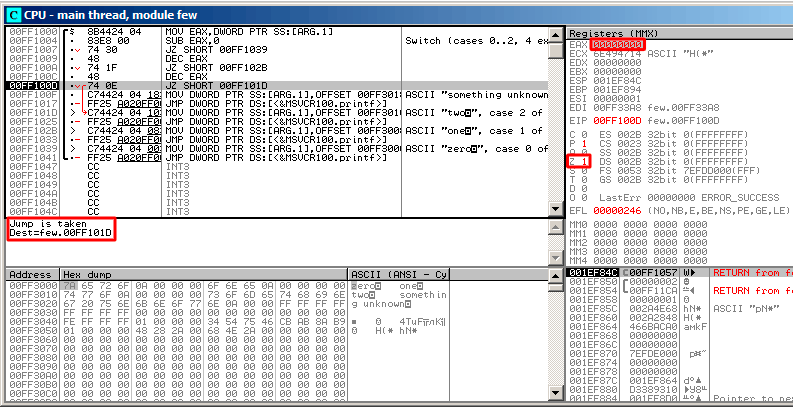
\includegraphics[scale=\FigScale]{patterns/08_switch/1_few/olly4.png}
\caption{\olly: вторая \DEC исполнилась}
\label{fig:switch_few_olly4}
\end{figure}

\olly показывает, что условный переход сейчас сработает.

\clearpage
Указатель на строку \q{two} 
сейчас будет записан в стек:

\begin{figure}[H]
\centering
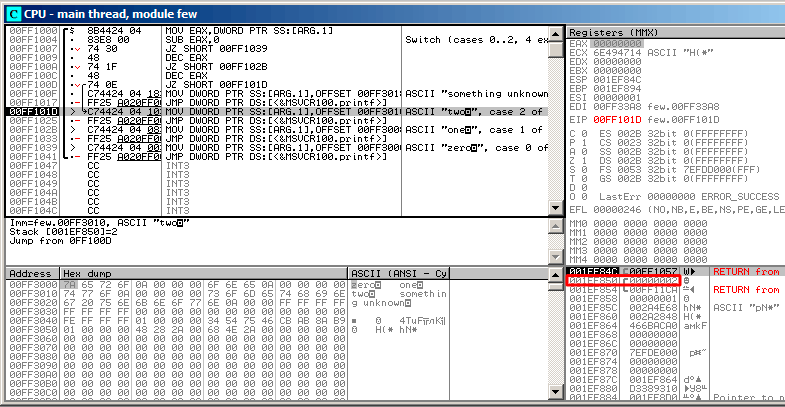
\includegraphics[scale=\FigScale]{patterns/08_switch/1_few/olly5.png}
\caption{\olly: указатель на строку сейчас запишется на место первого аргумента}
\label{fig:switch_few_olly5}
\end{figure}

% TODO: homogenize numbers
% now they are inconsistent: sometimes plain text, sometimes in math mode
% some kind of \expr{} both for numbers and expressions? --DY
Обратите внимание: текущий аргумент функции это 2 и 2 прямо сейчас в стеке по адресу \TT{0x001EF850}.

\clearpage
\MOV записывает указатель на строку по адресу \TT{0x001EF850} (см. окно стека).
Переход сработал.
Это самая первая инструкция функции \printf в MSVCR100.DLL (этот пример был скомпилирован с опцией /MD): 

\begin{figure}[H]
\centering
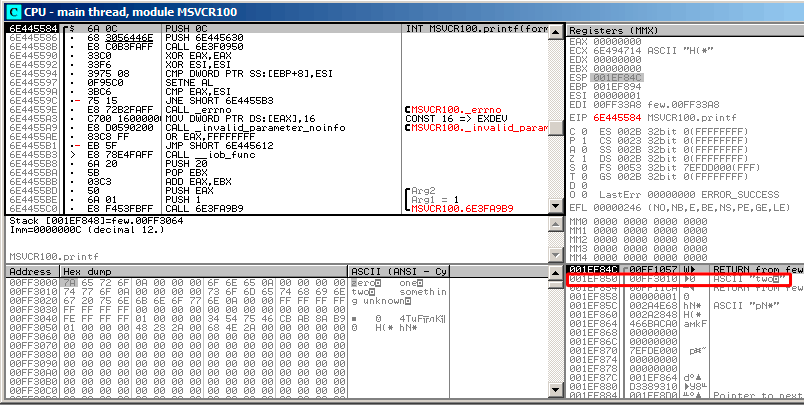
\includegraphics[scale=\FigScale]{patterns/08_switch/1_few/olly6.png}
\caption{\olly: первая инструкция в \printf в MSVCR100.DLL}
\label{fig:switch_few_olly6}
\end{figure}

Теперь \printf считает строку на \TT{0x00FF3010} как свой единственный аргумент и выводит строку.

\clearpage
Это самая последняя инструкция функции \printf:

\begin{figure}[H]
\centering
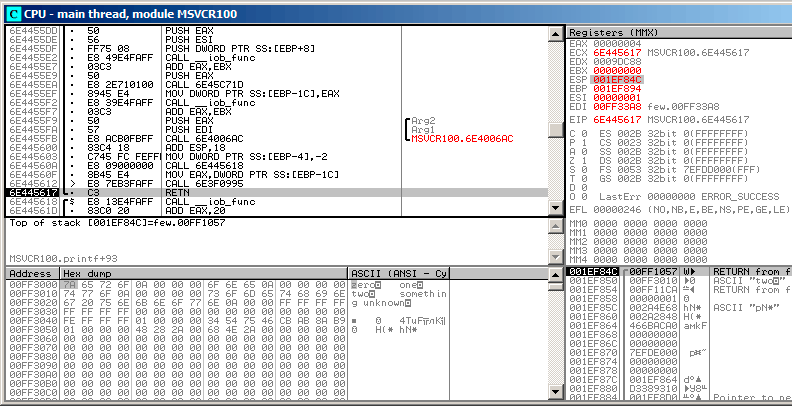
\includegraphics[scale=\FigScale]{patterns/08_switch/1_few/olly7.png}
\caption{\olly: последняя инструкция в \printf в MSVCR100.DLL}
\label{fig:switch_few_olly7}
\end{figure}

Строка \q{two} была только что выведена в консоли.

\clearpage
Нажмем F7 или F8 (\stepover) и вернемся\dots нет, не в функцию \ttf но в \main:

\begin{figure}[H]
\centering
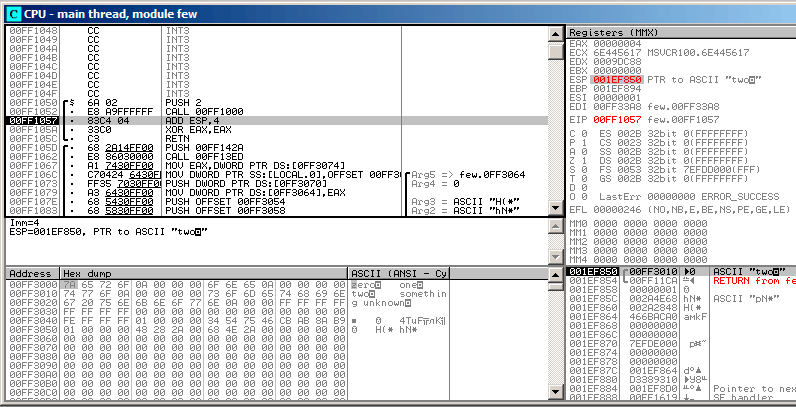
\includegraphics[scale=\FigScale]{patterns/08_switch/1_few/olly8.png}
\caption{\olly: возврат в \main}
\label{fig:switch_few_olly8}
\end{figure}

Да, это прямой переход из внутренностей \printf в \main.
Потому как \ac{RA} в стеке указывает не на какое-то место в функции \ttf а в \main.
И \CALL \TT{0x00FF1000} это инструкция вызывающая функцию \ttf.

